%%%%%%%%%%%%%%%%%%%%%%%%%%%%%%%%%%%%%%%%%%%%%%%%%%%%%%%%%%%%%%%%%%%
%                                                                 %
%                            CHAPTER THREE                        %
%                                                                 %
%%%%%%%%%%%%%%%%%%%%%%%%%%%%%%%%%%%%%%%%%%%%%%%%%%%%%%%%%%%%%%%%%%%

\chapter{CONCEPTUAL MODEL}\label{ch:model}

The goal of dataset versioning is to expose the relationships between versions of a dataset.
To do this, the concept model relates three kinds of objects, versions, attributes, and changes, with three kinds of changes, addition, invalidation, and modification.
To do this, we create a mapping between an original set and a new dataset.
As mentioned previously, the operations conducted by data versioning systems boil down to primarily three operations: addition, invalidation, and modification.
Since these operations are so prevalent, we use these three procedures to characterize the relationships between versions.
A modification is straight forward to model because it maps together two attributes of the version that exist, but addition and invalidation are a little different.
Because the item doesn't exist in one version or the other for addition and invalidation, it forms a '0 to 1' relationship between the attributes.
This causes a problem conceptually because without a concept on one end, there is nothing to connect on one end.
The chosen solution was to use the version concept as the anchor in place of the non-existant attribute.
This observation leads to the structure of the conceptual model used in this dissertation.
The construction of the relationship decides the kind of change that is occurring.
It then becomes easier to identify which change is occurring based off of whether attributes exist or not in which version.
In addition, while the figures in this chapter only show the attribute relationships as 0 to 1, 1 to 0, and 1 to 1, it is more valid to consider the relationships as 0 to X, X to 0, and X to Y in cardinality.
A modification may change a single location attribute into two separate latitude and longitude entries, for example.

From the discussion above, three kinds of objects appear: versions, attributes, and change.
That is to say we cannot properly represent versioning with versions alone.
The changes which we are interested in result from comparing the parts or attributes of the versions.
The Dublin Core Term hasPart provides a sufficient property to relate versions and their attributes together.
An observation that will not be further explored in this research is that attributes can also be versions.
For example, when comparing two revisions of a dataset, the attributes would be data files.
However, these files will be versions of each other, and their attributes will be, if tabular data, the rows of each file.
This nesting speaks towards the granularity by which an individual desires to perform version, but also demonstrates the challenge of using major and minor numbers to capture version change with the current dot-decimal identifier scheme.

An obvious concern about using this method of mapping, of finding attributes that are common and uncommon, between two or more objects is not unique two versioning.
In order to ensure that the relationships being exposed by the mapping is valid, we must go back to the definition of versions.
By requiring that the objects to have common provenance, we establish that performing a comparison to make a mapping compares related objects and information.
The second requirements, that the objects share the same workflow step, establishes that when we do make a mapping, that the attributes actually are the same.
This also addresses the possibility that we are comparing objects that have different purposes at separate points in a workflow, but share provenance as a result.

\section{MODIFICATION}

The simplest operation to model is Modification because it has no missing parts.
It maps a change from one attribute of version one to its corresponding attribute in version two.
In Figure \ref{ModificationFig}, a versioning comparison is being performed between two objects, Version 1 and Version 2.
Each version has an attribute, Attribute 1 and Attribute 2, respectively.
Finally, a change object connects the two attributes, denoting that the values described by the attribute are different.

Notice that the model captures neither the change's magnitude, nor the values of the attributes involved in the change.
These are not included because too much domain knowledge will be required to interpret the significance of the value.
In addition, the model would essentially begin storing a copy of the dataset, leading to space and redundancy concerns.
If an application needs to include this information, they can be added as a property of the attributes involved.
Simply knowing that the attribute has changed provides valuable information to identify the relationship between the two attributes from a versioning standpoint.
Sometimes it may be necessary to distinguish between modification changes.
For this reason, the change concept in this relationship may be sub-classed to differentiate between different kinds of change that map one attribute to another.
For example, in order to distinguish a modification in which the units of a measurement changes, a unit change concept, which sub-classes the modify change concept, can be used to connect the attributes from two different version.



\begin{figure}
	\centering
	\vspace{0.0in} % normally the command here would be \includegraphics
	%	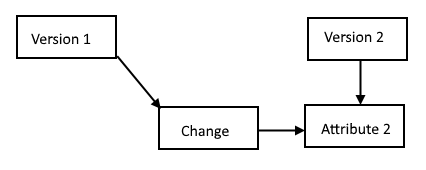
\includegraphics{figures/Addition.png}
	\begin{tikzpicture}[every node/.style={draw, rectangle}]
	\begin{scope}[node distance=20mm and 20mm]
	\node (c) [scale=1.25] at (1,0) {Change M};
	\node (1) [above left=of c, scale=1.25] {Version 1};
	\node (2) [above right=of c, scale=1.25] {Version 2};
	\node (a1) [below =of 1, scale=1.25] {Attribute 1};
	\node (a2) [below =of 2, scale=1.25] {Attribute 2};
	
	\draw [line width=2pt,->] (a1) -- (c);
	\draw [line width=2pt,->] (c) -- (a2);
	\draw [line width=2pt, ->] (1) -- (a1);
	\draw [line width=2pt, ->] (2) -- (a2);
	\end{scope}
	\end{tikzpicture}
	\caption{Model of the relationships between Versions 1 and 2 when modifying Attribute 1 from Version 1 as a result of Change M, resulting in Attribute 2 from Version 2}
	\label{ModificationFig}  % the \label command comes AFTER the caption
\end{figure}

\section{ADDITION}

When discussing additions, a new attribute is added to version one, leading to its appearance as an attribute in version two.
In this case, it makes sense that since the attribute is not in version one, then it should not appear on that version's side in the model.

When a change adds a new attribute to a version, it only needs to refer to version two and its corresponding attribute.  The reasoning should be fairly obvious as the attribute never existed in version one, and therefore, there is nothing to refer to and no need to form a relationship between the change and version one.  However, by linking the addition change to version one, we address a difficulty with comparing provenance graphs.  When two data objects have identical structures, it is difficult to determine what time the objects were added to the dataset and which version they belong to.  As a result, determining the compatability of the two objects becomes difficult.  The change contributions to the dataset evolution appears naturally using this construction. The resulting model can be seen in Figure~\ref{AdditionFig}.  Some relationships are specifically left out, such as that between Change A and Version 2, to not confuse identification of other types of changes.  The relationship between Change A and Version 2 can still be implied from Attribute 2.

\begin{figure}
	\centering
	\vspace{0.0in} % normally the command here would be \includegraphics
%	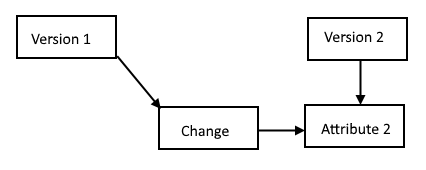
\includegraphics{figures/Addition.png}
	\begin{tikzpicture}[every node/.style={draw, rectangle}]
		\begin{scope}[node distance=20mm and 20mm]
			\node (c) [scale=1.25] at (1,0) {Change A};
			\node (1) [above left=of c, scale=1.25] {Version 1};
			\node (2) [above right=of c, scale=1.25] {Version 2};
			\node (a) [below =of 2, scale=1.25] {Attribute 2};
			
			\draw [line width=2pt,->] (1) -- (c);
			\draw [line width=2pt,->] (c) -- (a);
			\draw [line width=2pt, ->] (2) -- (a);
		\end{scope}
	\end{tikzpicture}
	\caption{Model of the relationships between Versions 1 and 2 when adding an Attribute 2 to Version 2 as a result of Change A}
	\label{AdditionFig}  % the \label command comes AFTER the caption
\end{figure}


\section{INVALIDATION}

The invalidation relationship has a missing attribute object on the other side of the relation, contrary to the addition construction.
As a result of the invalidation, an attribute no longer exists in the following version.
As seen in Figure \ref{InvalidationFig}, the invalidation change concept matches to the Version 2 object.
Just like in addition model, this construction maintains a link between the two version objects.
However, in this case, it makes more conceptual sense because Version 2 invalidates Attribute 1 by omitting it.

Related concepts include Schema.org's DeleteAction and PROV's Invalidation.
PROV defines the property as the "start of the destruction, cessation, or expiry of an existing entity by an activity," but since nothing actively creates versioning relationships, this property is inappropriate for this application \cite{Lebo2013}.
There is no activity to credit with removing the property in this comparison, and the absence results from a state-based property.
Schema.org defines the DeleteAction as, "The act of editing a recipient by removing one of its objects," \cite{SchemaRem}.
This definition assumes that an actor will perform an action upon an object or collection, removing one of its members, producing a new result.
This follows the provenance mentality, but when versioning, the resulting object has already been created.
Cases exist, as shown in Chapter 4, where an attribute is not included in a new version, thus indicating that it has been removed.
However, the most important point of contention in this definition is the idea of removal and deletion.
Although an object is no longer valid, it does not mean the data has been deleted.
Invalid data often gets removed, but this is not always the case.
As a result, naming the concept invalidation is more general and inclusive.

\begin{figure}
	\centering
	\vspace{0.0in} % normally the command here would be \includegraphics
	%	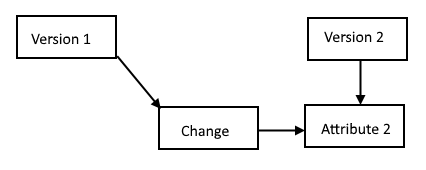
\includegraphics{figures/Addition.png}
	\begin{tikzpicture}[every node/.style={draw, rectangle}]
	\begin{scope}[node distance=15mm and 20mm]
	\node (c) [scale=1.25] at (1,0) {Change I};
	\node (1) [above left=of c, scale=1.25] {Version 1};
	\node (2) [above right=of c, scale=1.25] {Version 2};
	\node (a) [below =of 1, scale=1.25] {Attribute 1};
	
	\draw [line width=2pt,->] (a) -- (c);
	\draw [line width=2pt,->] (c) -- (2);
	\draw [line width=2pt, ->] (1) -- (a);
	\end{scope}
	\end{tikzpicture}
	\caption{Model of the relationships between Versions 1 and 2 when invalidating Attribute 1 from Version 1 as a result of Change I}
	\label{InvalidationFig}  % the \label command comes AFTER the caption
\end{figure}



\section{MULTIPLE LINKED VERSIONS}

Using the construction outlined in the previous three sections, many changes can be compiled together into a graph in a changelog.  After all additions, invalidations, and modifications have been compiled into a single graph, a complete mapping from version one to version two may be developed.  The orientation of the relationships in the graph allows a flow to be created from attributes in version one to corresponding attributes in version two.  Taking version two and performing the same graph construction to a version three results in not only a flow from version two to version three, but also from version one to version three.  As a result, the flow can be used to construct a mapping from version one to version three or any future version.
